%\section{Percepção dos desenvolvedores em relação às vulnerabilidades em aplicativos open source}

%Este trabalho considera a percepção dos desenvolvedores e profissionais de segurança em relação às vulnerabilidades em aplicativos open source. O estudo não se limitou apenas à análise estática das ferramentas utilizadas, mas também incluiu uma investigação sobre aplicativos Android de código aberto, com o objetivo de obter a opinião dos desenvolvedores envolvidos.

%Uma descoberta relevante foi que muitas das questões identificadas pelo CogniCrypt não estavam diretamente relacionadas ao código do aplicativo Android em si, mas sim às bibliotecas de terceiros utilizadas por esses aplicativos. Dentre os projetos de código aberto analisados, aproximadamente 60\% apresentaram questões levantadas pelo CogniCrypt que se originavam de códigos de terceiros. Os desenvolvedores abordaram essas preocupações de segurança de maneiras diversas. Alguns optaram por atualizar imediatamente as dependências, enquanto outros confiaram implicitamente nas grandes empresas de tecnologia fornecedoras das bibliotecas e não consideraram os problemas como ameaças reais.

%Em alguns casos, os desenvolvedores tiveram dificuldades em compreender completamente as questões apresentadas pelo CogniCrypt. Para eles, não estava claro por que determinados trechos de código eram considerados problemas apenas a partir das explicações fornecidas pela ferramenta. Diante disso, os desenvolvedores expressaram o desejo de receber explicações mais detalhadas sobre os problemas identificados, bem como sugestões diretas sobre como corrigi-los. Além disso, alguns sugeriram a categorização dos problemas levantados pelo CogniCrypt com base na origem, indicando se pertencem ao aplicativo digitalizado ou a uma biblioteca de terceiros. Essa observação proporciona insights valiosos sobre a necessidade de uma comunicação mais eficaz entre as ferramentas de análise e os desenvolvedores, visando uma compreensão mais precisa e eficiente das vulnerabilidades detectadas.

\section{RQ1. Quantidade de warnings encontrados pelas ferramentas CogniCrypt e CryptoGuard}

Foram analisados 307 aplicativos de 6 diferentes categorias do repositório de aplicativos de código aberto F-Droid. A execução do CogniCrypt reportou 195 \textit{warnings} de uso indevido de criptografia, enquanto o CryptoGuard reportou 298. A tabela abaixo mostra a quantidade de aplicativos analisados por categoria e a quantidade de \textit{warnings} reportados por cada ferramenta.

\begin{table}[!htbp]
  \centering
  \begin{tabular}{|c|c|c|c|}
  
    \textbf{Categoria}   & \textbf{Número de Aplicativos}   &  \textbf{CogniCrypt}     &  \textbf{CryptoGuard} \\ 
     Connectivity           & \num{58}                         &  \num{20}                    & \num{3}                     \\
Finances                & \num{90}                         &  \num{25}                    & \num{2}                     \\
Internet                 & \num{39}                         &  \num{7}                      &     \num{0}                  \\
Security                 & \num{47}                         &  \num{16}                    &     \num{1}                  \\
Sms-Phone            & \num{18}                         &  \num{10}                     &     \num{2}                 \\
System                  & \num{55}                        &   \num{34}                    &     \num{0}                  \\
\textbf{Total}        & \num{307}                      &   \num{112}                  &     \num{8}                   \\
\end{tabular}
    
  \caption{Aplicativos por categoria sem warning das ferramentas CogniCrypt e CryptoGuard}
\label{AplicativosSemWarning}
\end{table}

Como visto, o número de aplicativos sem \textit{warnings} no CogniCrypt é bem maior do que no CryptoGuard. A categoria Sistema é a que apresenta a maior diferença entre eles, com \num{34} aplicativos. As categorias Conectividade e Finanças também têm um número elevado de aplicativos sem \textit{warnings}, \num{20} e \num{25}, respectivamente.

Apesar disso, o número de \textit{warnings} encontrados pelo CogniCrypt é maior do que no CryptoGuard, conforme descrito na tabela abaixo.

\begin{table}[!htbp]
  \centering
  \begin{tabular}{|c|c|c|c|}
  
\textbf{Categoria}   & \textbf{CogniCrypt (a)}   &  \textbf{CryptoGuard (b)}     &  \textbf{Diferença (a - b)} \\ 
Connectivity           & \num{1768} (\num{16.02}\%)  &  \num{1124} (\num{22.64}\%)  & \num{644} (\num{10.61}\%) \\
Finances                &     \num{3087} (\num{27.97}\%)     &     \num{1687} (\num{33.98}\%)     &     \num{1400} (\num{23.06}\%)\\
Internet                 &     \num{3407} (\num{30.87}\%)     &     \num{916} (\num{18.45}\%)     &     \num{2491} (\num{41.02}\%)\\
Security                 &     \num{1780} (\num{16.13}\%)     &     \num{553} (\num{11.14}\%)     &     \num{1227} (\num{20.21}\%)\\
Sms-Phone            &     \num{428} (\num{3.88}\%)     &     \num{171} (\num{3.44}\%)     &     \num{257} (\num{4.23}\%)\\
System                  &     \num{566} (\num{5.13}\%)     &     \num{513} (\num{10.33}\%)     &     \num{53} (\num{0.87}\%)\\
\textbf{Total}                     &     \num{11036} (\num{100.00}\%)     &     \num{4964} (100.00\%)     &     \num{6072} (\num{100.00}\%)\\
\end{tabular}
    
  \caption{Warnings encontrados nas ferramentas CogniCrypt e CryptoGuard}
\label{AplicativosComWarning}
\end{table}

Como podemos observar na tabela acima, o CogniCrypt conseguiu encontrar \num{4964} \textit{warnings}, enquanto o CryptoGuard encontrou \num{11036} \textit{warnings}. A diferença numérica é de \num{6072} (ou \num{122.32}\%) \textit{warnings} entre as duas ferramentas. As categorias de Finanças e Internet concentraram \num{58.8}\% (\num{6494}) dos \textit{warnings} do CogniCrypt, enquanto as categorias de Finanças e Conectividade concentraram \num{56.6}\% (\num{2811}) dos \textit{warnings} do CryptoGuard. A maior diferença entre os \textit{warnings} encontrados foi notada nas categorias Internet (\num{2491}) e Finanças (\num{1400}), representando \num{64.1}\% de diferença.

\subsection{RQ2 e RQ3. Quantidade de warnings de bibliotecas externas e possivelmente externas}

A fim de facilitar a análise, os aplicativos foram categorizados. Em cada categoria, serão exibidos os resultados relativos ao número de aplicativos com alertas de vulnerabilidade, diferenciando aqueles que são potencialmente externos dos que são definitivamente externos, para cada ferramenta utilizada. As tabelas a seguir apresentam os resultados dessas integrações.

\textbf{CogniCrypt}

\begin{table}[!htbp]
  \centering
  \small
  \begin{tabular}{|c|c|c|c|c|}
  
\textbf{CC/Connectivity}   & \textbf{Warnings (a)}   &  \textbf{Possible ext (b)}     &  \textbf{Definite ext (c)} &  \textbf{Native-ext (a-b-c)} \\ 
Média                      & \num{21.9}              &  \num{2.3}                                         & \num{2.4}                                        & \num{17.1}                                                    \\
Desvio Padrão              & \num{43.8}              &  \num{10.3}                                         & \num{6.1}                                        & \num{42.8}                                 \\                    
Variância                  & \num{1919.8}            &  \num{107.8}                                         & \num{38.2}                                       & \num{1831.9}         \\                                           
\end{tabular}
    
  \caption{Resultados da integração do CogniCrypt com o LibScout na categoria Connectivity}
\label{table: AplicativosComWarningCCC}
\end{table}


\begin{table}[!htbp]
  \centering
  \small
  \begin{tabular}{|c|c|c|c|c|}
  
\textbf{CC/Finances}   & \textbf{Warnings (a)}   &  \textbf{Possible ext (b)}     &  \textbf{Definite ext (c)} &  \textbf{Native-ext (a-b-c)} \\ 
Média                      & \num{46.4}          &  \num{2.8}                                                  & \num{7.5}                                         & \num{35.9}                                                    \\
Desvio Padrão              & \num{132.06}           &  \num{10.8}                                                 & \num{41.8}                                        & \num{126.07}          \\                                          
Variância                  & \num{17439.9}       &  \num{118.2}                                                & \num{1747.7}                                      & \num{15895.3}    \\                                                
\end{tabular}
    
  \caption{Resultados da integração do CogniCrypt com o LibScout na categoria Finances}
\label{table: AplicativosComWarningCCF}
\end{table}


\begin{table}[!htbp]
  \centering
  \small
  \begin{tabular}{|c|c|c|c|c|}
  
\textbf{CC/SMS}   & \textbf{Warnings (a)}   &  \textbf{Possible ext (b)}     &  \textbf{Definite ext (c)} &  \textbf{Native-ext (a-b-c)} \\ 
Média                      & \num{11.7}              &  \num{2.36}                                         & \num{1}                                        & \num{8.3}                                                    \\
Desvio Padrão              & \num{31.67}              &  \num{7.78}                                         & \num{3.69}                                        & \num{24.1}   \\                                                 
Variância                  & \num{1003.03}            &  \num{60.54}                                         & \num{12.94}                                       & \num{585.4}             \\                                       
\end{tabular}
    
  \caption{Resultados da integração do CogniCrypt com o LibScout na categoria SMS}
\label{table: AplicativosComWarningCCSMS}
\end{table}


\begin{table}[!htbp]
  \centering
  \small
  \begin{tabular}{|c|c|c|c|c|}
  
\textbf{CC/System}   & \textbf{Warnings (a)}   &  \textbf{Possible ext (b)}     &  \textbf{Definite ext (c)} &  \textbf{Native-ext (a-b-c)} \\ 
Média                      & \num{10.09}              &  \num{0.93}                                         & \num{0.36}                                        & \num{8.79}                                                    \\
Desvio Padrão              & \num{33.01}              &  \num{3.74}                                         & \num{1.28}                                        & \num{31.82}  \\                                                  
Variância                  & \num{1090.2}            &  \num{14.05}                                         & \num{1.66}                                       & \num{1012.5}  \\                                                  
\end{tabular}
    
  \caption{Resultados da integração do CogniCrypt com o LibScout na categoria System}
\label{table: AplicativosComWarningCCS}
\end{table}

Os resultados para a tabela de conectividade (\ref{table: AplicativosComWarningCCC}) mostram que, em média, por aplicativo, o CogniCrypt encontrou \num{21.9} \textit{warnings} de vulnerabilidade. Desses, \num{2.3} são possivelmente externos e \num{2.4} são definitivamente externos. A quantidade de \textit{warnings} nativos é de \num{17.1}.
Para finanças (\ref{table: AplicativosComWarningCCF}), a média de \textit{warnings} por aplicativo é de \num{46.4}. Desses, \num{2.8} são possivelmente externos e \num{7.5} são definitivamente externos. A quantidade de \textit{warnings} nativos é de \num{35.9}. 
Para SMS (\ref{table: AplicativosComWarningCCSMS}), a média de \textit{warnings} por aplicativo é de \num{11.7}. Desses, \num{2.36} são possivelmente externos e \num{1} é definitivamente externo. A quantidade de \textit{warnings} nativos é de \num{8.3}.
E para sistema (\ref{table: AplicativosComWarningCCS}), a média de \textit{warnings} por aplicativo é de \num{10.09}. Desses, \num{0.93} são possivelmente externos e \num{0.36} são definitivamente externos. A quantidade de \textit{warnings} nativos é de \num{8.79}.
Em todos os exemplos, o desvio padrão e a variância são altos, indicando que os valores estão bem dispersos. Isso é explicado tanto pelas limitações do LibScout quanto pelas limitações do CogniCrypt. O LibScout pode não ter mapeado a biblioteca com \textit{warning} como externa, e o CogniCrypt pode ter encontrado \textit{warnings} em bibliotecas que não foram mapeadas pelo LibScout ou ainda não ter encontrado vulnerabilidade no aplicativo selecionado.

\textbf{CryptoGuard}

\begin{table}[!htbp]
  \centering
  \small
  \begin{tabular}{|c|c|c|c|c|}
    \hline
    \textbf{CG/Connectivity} & \textbf{Total Libraries} & \textbf{Possible Ext.} & \textbf{Definite Ext.} & \textbf{Native Libraries} \\
    \hline
    Média & \num{15.1} & \num{0.73} & \num{5.21} & \num{9.22} \\
    Desvio Padrão & \num{25.62} & \num{2.17} & \num{9.91} & \num{18.7} \\
    Variância & \num{656.6} & \num{4.71} & \num{98.3} & \num{352.4} \\
    \hline
  \end{tabular}
  \caption{Resultados da integração do CryptoGuard com o LibScout na categoria Connectivity}
  \label{table: AplicativosComWarningCGC}
\end{table}


\begin{table}[!htbp]
  \centering
  \small
  \begin{tabular}{|c|c|c|c|c|}
    \hline
    \textbf{CG/Finances} & \textbf{Total Libraries} & \textbf{Possible Ext.} & \textbf{Definite Ext.} & \textbf{Native Libraries} \\
    \hline
    Média & \num{10.45} & \num{1.33} & \num{4.68} & \num{4.43} \\
    Desvio Padrão & \num{20.71} & \num{4.72} & \num{10.03} & \num{10.05} \\
    Variância & \num{429.13} & \num{22.2} & \num{100.72} & \num{101.1} \\
    \hline
  \end{tabular}
  \caption{Resultados da integração do CryptoGuard com o LibScout na categoria Finances}
  \label{table: AplicativosComWarningCGF}
\end{table}


\begin{table}[!htbp]
  \centering
  \small
  \begin{tabular}{|c|c|c|c|c|}
    \hline
    \textbf{CG/SMS} & \textbf{Total Libraries} & \textbf{Possible Ext.} & \textbf{Definite Ext.} & \textbf{Native Libraries} \\
    \hline
    Média & \num{9} & \num{0.78} & \num{2.73} & \num{5.47} \\
    Desvio Padrão & \num{18.72} & \num{2.09} & \num{5.66} & \num{16.22} \\
    Variância & \num{350.6} & \num{4.37} & \num{32.08} & \num{263.19} \\
    \hline
  \end{tabular}
  \caption{Resultados da integração do CryptoGuard com o LibScout na categoria SMS}
  \label{table: AplicativosComWarningCGSMS}
\end{table}


\begin{table}[!htbp]
  \centering
  \small
  \begin{tabular}{|c|c|c|c|c|}
    \hline
    \textbf{CG/System} & \textbf{Total Libraries} & \textbf{Possible Ext.} & \textbf{Definite Ext.} & \textbf{Native Libraries} \\
    \hline
    Média & \num{7.53} & \num{0.65} & \num{2.67} & \num{4.2} \\
    Desvio Padrão & \num{16.49} & \num{2.69} & \num{7.07} & \num{12} \\
    Variância & \num{272.21} & \num{7.27} & \num{50.07} & \num{146.4} \\
    \hline
  \end{tabular}
  \caption{Resultados da integração do CryptoGuard com o LibScout na categoria System}
  \label{table: AplicativosComWarningCGS}
\end{table}

Analisando a tabela de conectividade (\ref{table: AplicativosComWarningCGC}), observa-se que o CryptoGuard, em média por aplicativo, detectou \num{15.1} alertas de vulnerabilidade, dos quais \num{0.73} são potencialmente externos e \num{5.21} definitivamente externos, com \num{9.22} alertas nativos. 
Na categoria de finanças (\ref{table: AplicativosComWarningCGF}), a média foi de \num{10.45} alertas por aplicativo, com \num{1.33} potencialmente externos e \num{4.68} definitivamente externos, além de \num{4.43} nativos.
Para SMS (\ref{table: AplicativosComWarningCGSMS}), a média foi de \num{9} alertas, com \num{0.78} potencialmente externos e \num{2.73} definitivamente externos, e \num{5.47} nativos.
E para sistema (\ref{table: AplicativosComWarningCGS}), a média foi de \num{7.53} alertas, com \num{0.65} potencialmente externos e \num{2.67} definitivamente externos, além de \num{4.2} nativos. 
Os altos desvios padrão e variância indicam uma dispersão significativa, influenciada pelas limitações do LibScout e do CryptoGuard. O LibScout pode não ter mapeado a biblioteca com \textit{warning} como externa, e o CryptoGuard pode ter encontrado \textit{warnings} em bibliotecas que não foram mapeadas pelo LibScout ou ainda não ter encontrado vulnerabilidade no aplicativo selecionado.


\begin{table}[!htbp]
  \centering
  \small
  \begin{tabular}{|c|c|c|}
    \hline
    \textbf{-} & \textbf{CogniCrypt} & \textbf{Cryptoguard} \\
    \hline
    Total Aplicativos & \num{246} & \num{253} \\
    Total Bibliotecas & \num{6798} & \num{2710}  \\
    Total Bibliotecas Externas & \num{1710} & \num{1149} \\
    Total Bibliotecas Externas Potenciais & \num{726} & \num{245} \\
    Total Bibliotecas Nativas & \num{4362} & \num{1316} \\
    \hline
  \end{tabular}
  \caption{Resultados da integração do CryptoGuard com o LibScout na categoria System}
  \label{table: AplicativosComWarningSummary}
\end{table}

A tabela \ref{table: AplicativosComWarningSummary} mostra um resumo dos resultados obtidos nas categorias analisadas. O CogniCrypt analisou 246 aplicativos, com 6798 bibliotecas, das quais 1710 são externas, 726 potencialmente externas e 4362 nativas. O CryptoGuard analisou 253 aplicativos, com 2710 bibliotecas, das quais 1149 são externas, 245 potencialmente externas e 1316 nativas.

\begin{figure}[!ht]
  \centering
  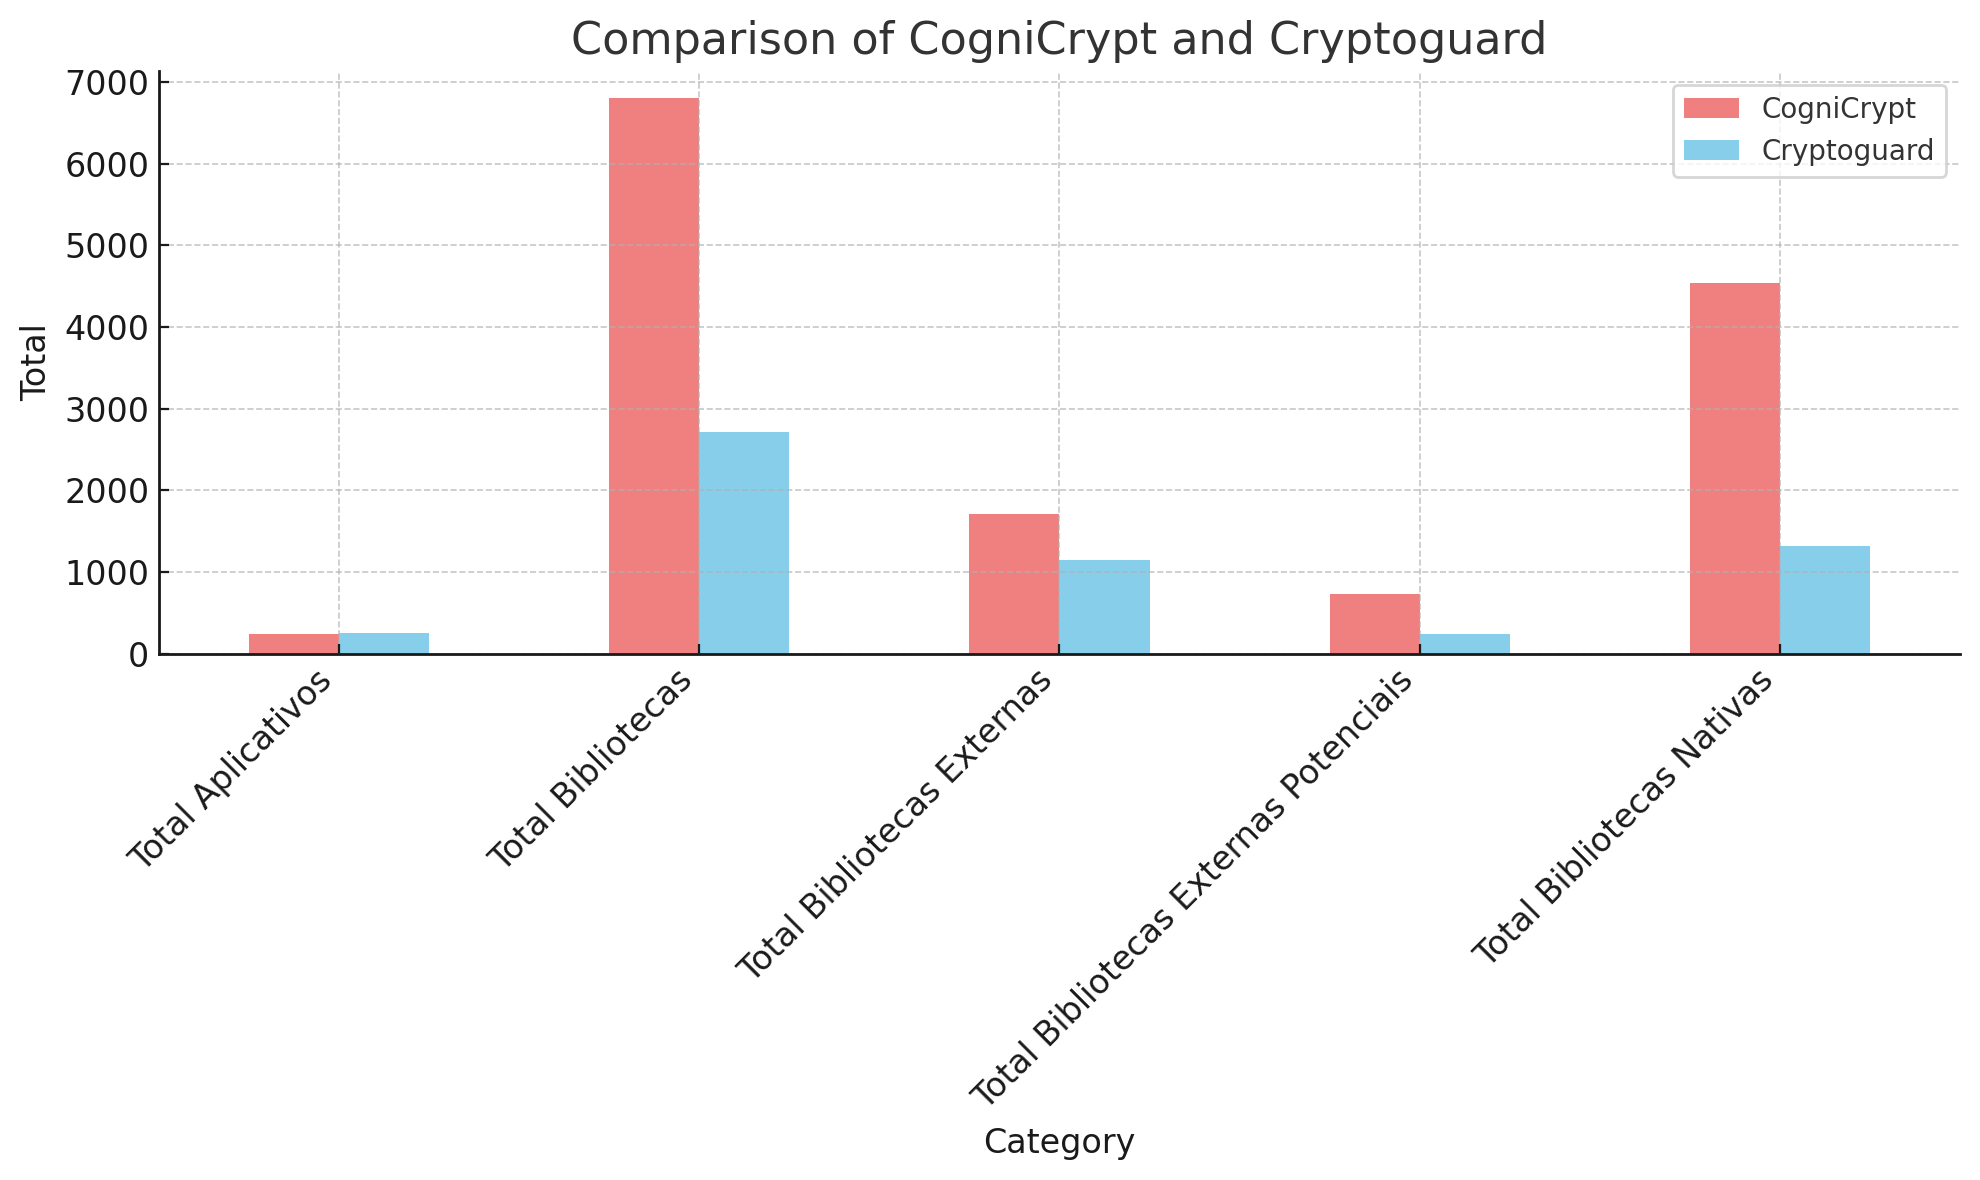
\includegraphics[scale=0.7]{img/plot_cc_x_cg_summary.png}
  \caption{Comparação total entre as ferramentas CogniCrypt e CryptoGuard}
  \label{img: CCvsCG_Summary}
\end{figure}

\begin{figure}[!ht]
  \centering
  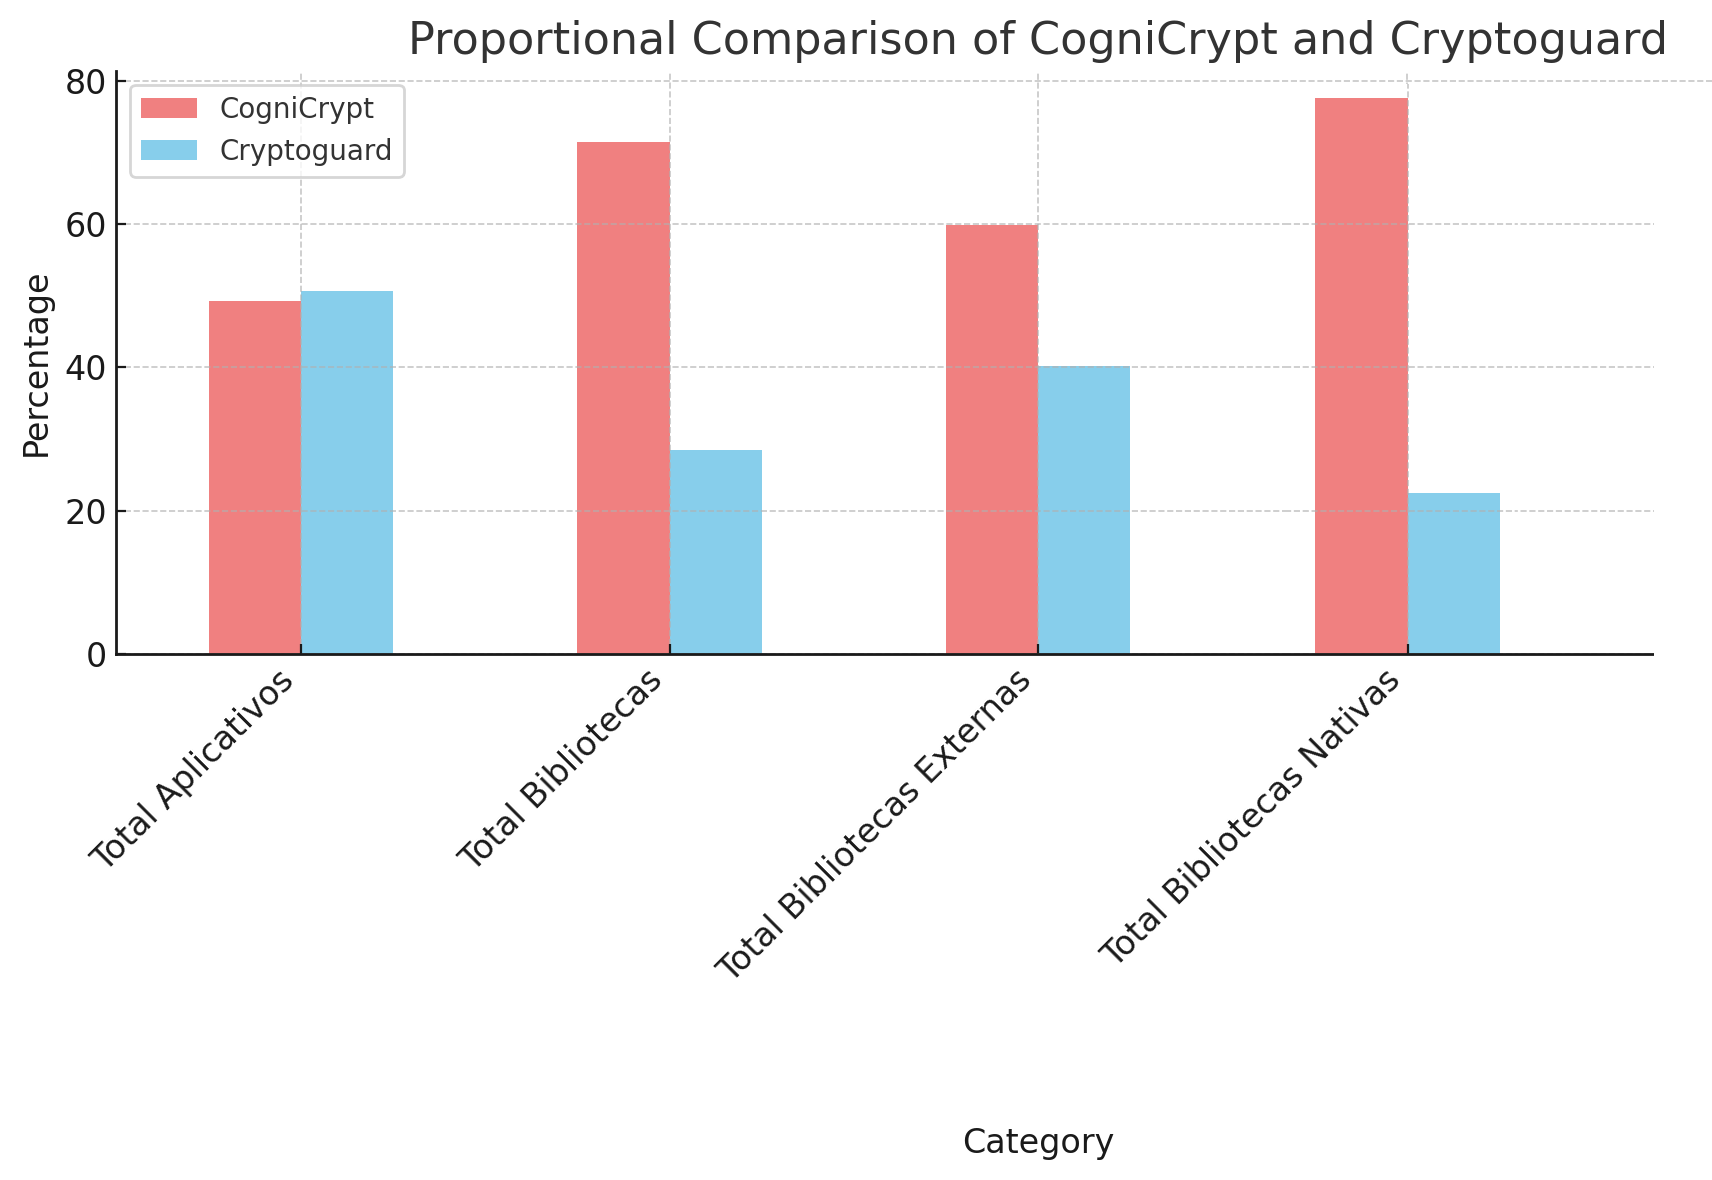
\includegraphics[scale=0.7]{img/plot_cc_x_cg_proportion_summary.png}
  \caption{Comparação proporcional total entre as ferramentas CogniCrypt e CryptoGuard}
  \label{img: CCvsCG_Summary2}
\end{figure}

Os resultados para a ferramenta CogniCrypt se destacaram em relação aos resultados para o CryptoGuard. 

\subsection{Resultados CogniCrypt x CryptoGuard}

As figuras subsequentes ilustram uma análise comparativa categorizada entre as ferramentas CogniCrypt e CryptoGuard


\begin{figure}[!ht]
  \centering
  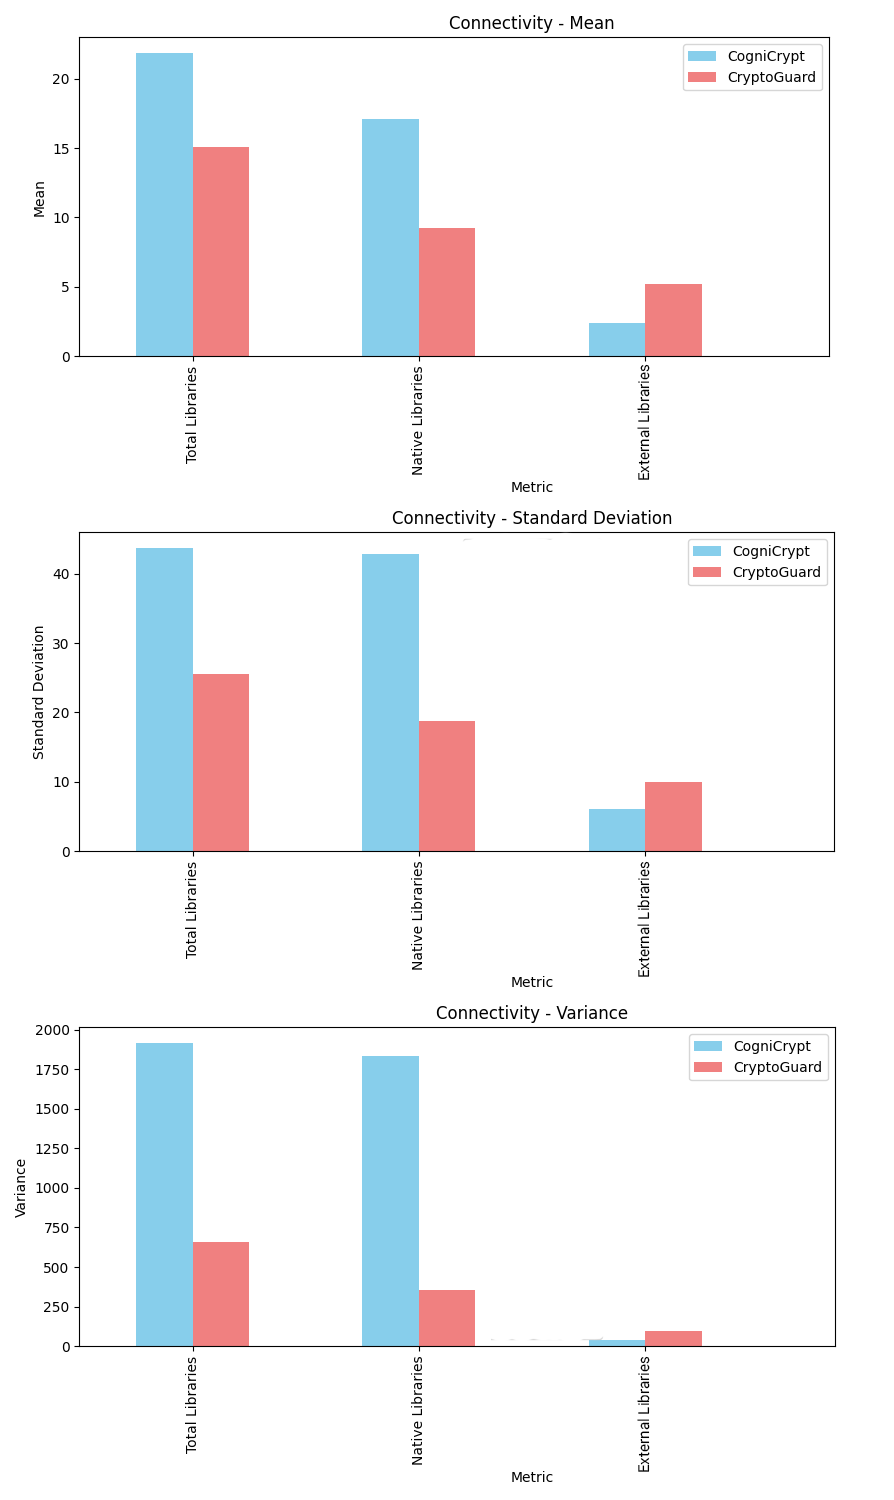
\includegraphics[scale=0.7]{img/plot_cc_x_cg_connectivity.png}
  \caption{Comparação entre as ferramentas CogniCrypt e CryptoGuard na categoria Connectivity}
  \label{img: CCvsCG_Connectivity}
\end{figure}

Na categoria de conectividade (\ref{img: CCvsCG_Connectivity}), a média de alertas emitidos pelas ferramentas indica que o CogniCrypt gera um número maior de alertas por aplicativo, incluindo alertas nativos e potencialmente externos. Contudo, o CryptoGuard excede no número de alertas definitivamente classificados como externos.
O CogniCrypt apresenta um desvio padrão e uma variância superiores, com exceção da quantidade de alertas de bibliotecas categorizadas como definitivamente externas.
A eficiência na integração com o LibScout, para a identificação de bibliotecas definitivamente externas, é mais pronunciada no CryptoGuard.

\begin{figure}[!ht]
    \centering
    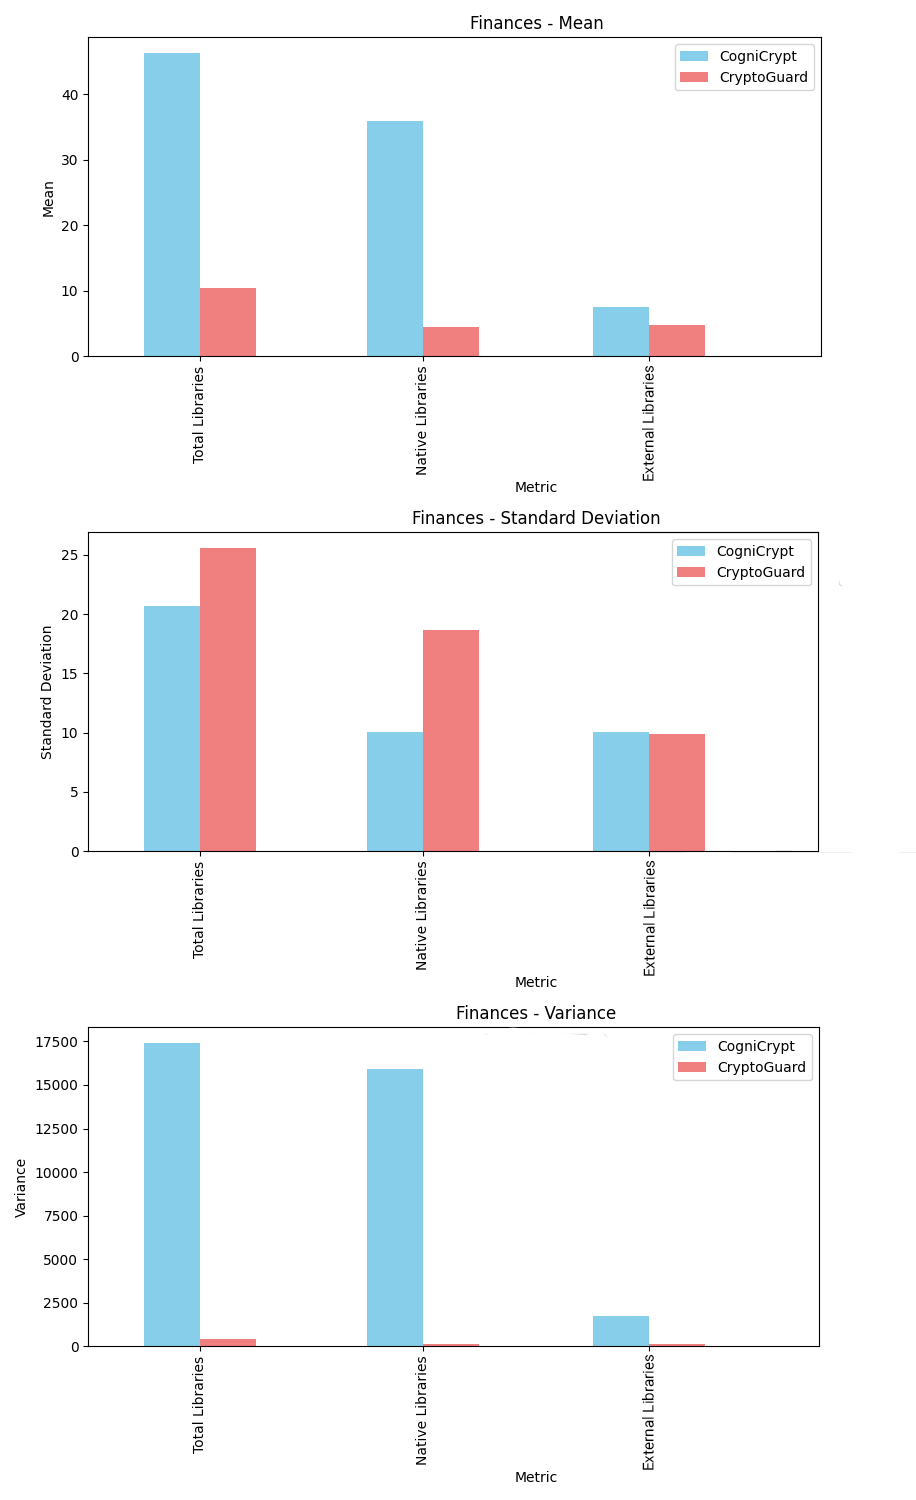
\includegraphics[scale=0.7]{img/plot_cc_x_cg_finances.png}
    \caption{Comparação entre as ferramentas CogniCrypt e CryptoGuard na categoria Finances}
    \label{img: CCvsCG_Finances}
\end{figure}

Na categoria financeira  (\ref{img: CCvsCG_Finances}), o CogniCrypt demonstrou superioridade em relação ao CryptoGuard.
Isso indica que o CryptoGuard tem uma dispersão maior nos valores relativos aos alertas por aplicativo e aos alertas de bibliotecas nativas, em contraste com a maior dispersão do CogniCrypt nos valores de alertas possivelmente de bibliotecas externas e definitivamente externas.



\begin{figure}[!ht]
    \centering
    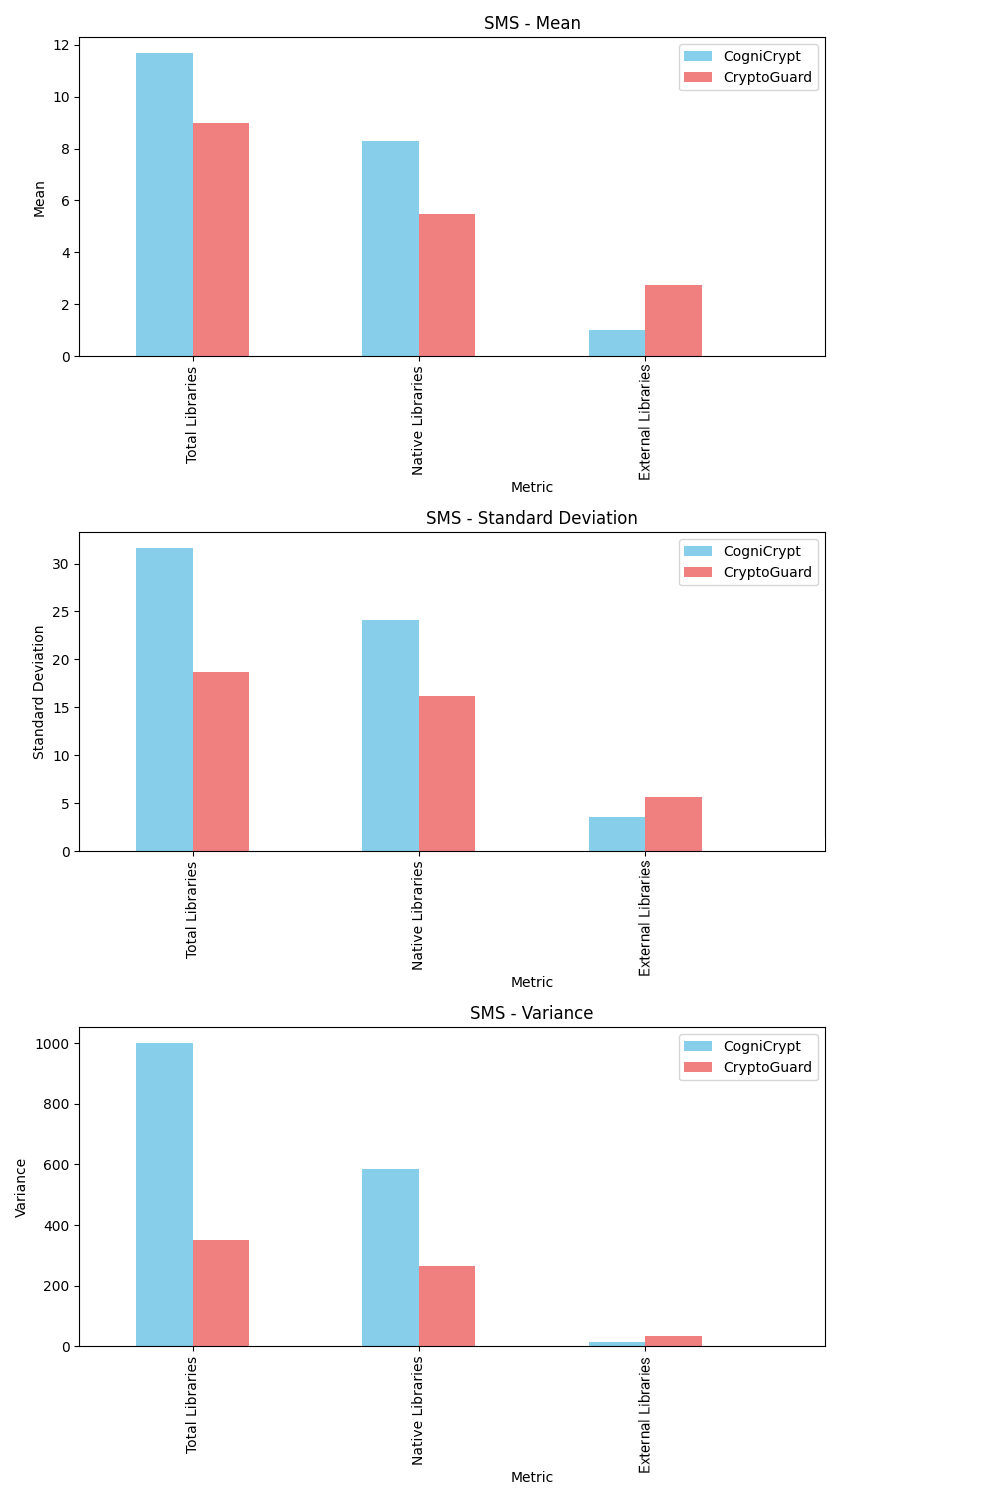
\includegraphics[scale=0.7]{img/plot_cc_x_cg_sms.png}
    \caption{Comparação entre as ferramentas CogniCrypt e CryptoGuard na categoria SMS}
    \label{img: CCvsCG_SMS}
\end{figure}

\begin{figure}[!ht]
    \centering
    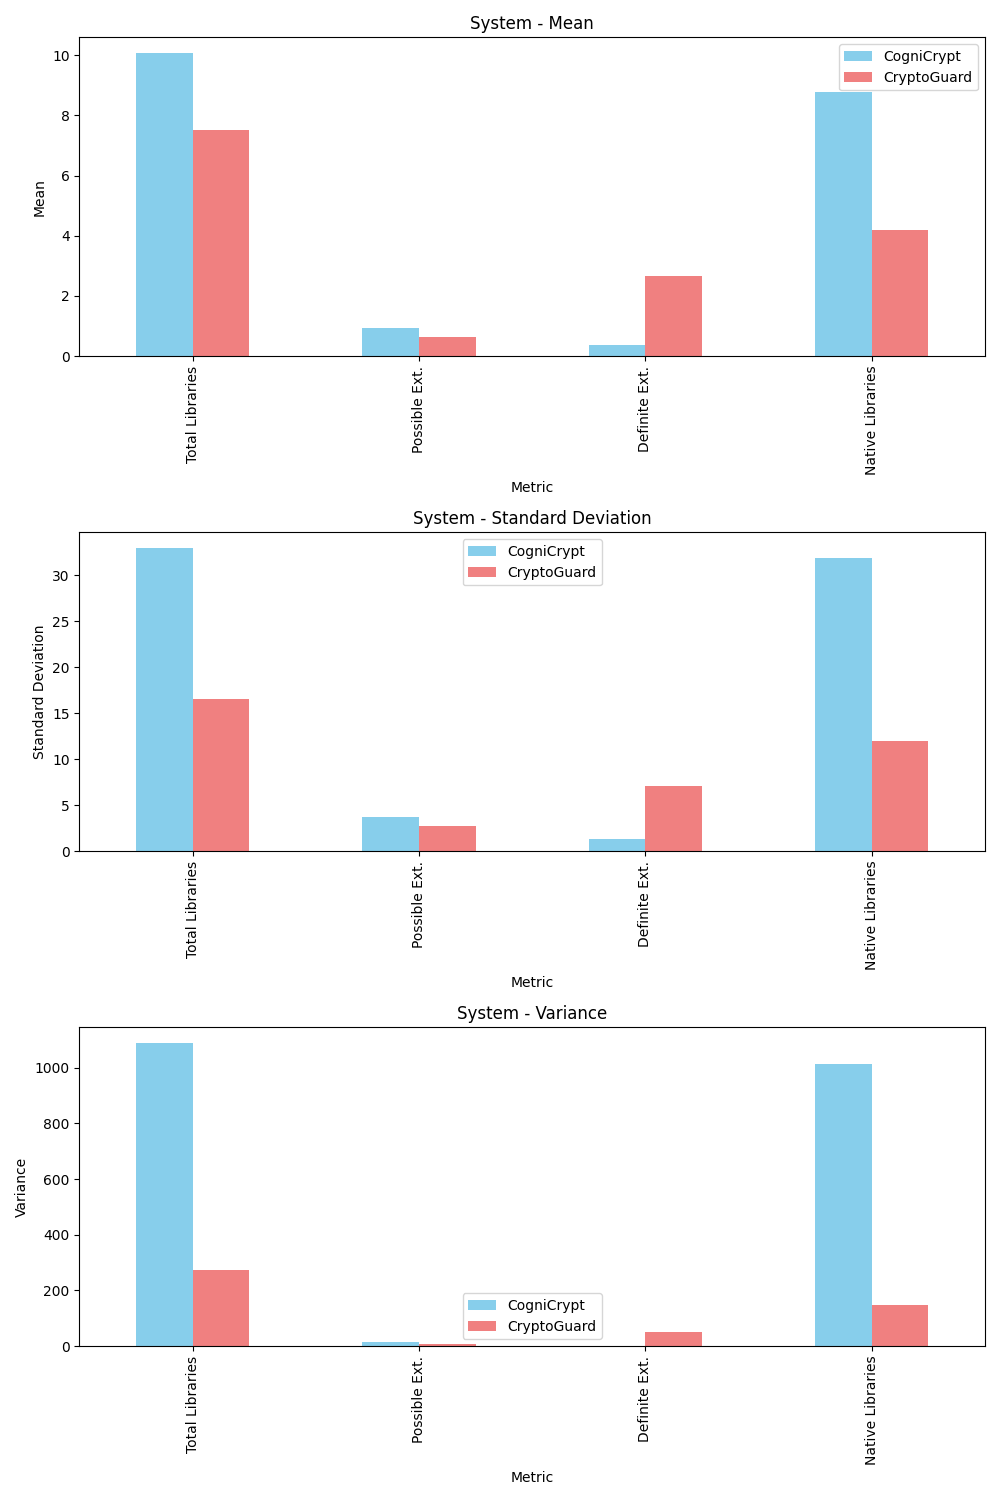
\includegraphics[scale=0.7]{img/plot_cc_x_cg_system.png}
    \caption{Comparação entre as ferramentas CogniCrypt e CryptoGuard na categoria System}
    \label{img: CCvsCG_System}
\end{figure}

Nas categorias de SMS (\ref{img: CCvsCG_SMS}) e Sistemas (\ref{img: CCvsCG_System}), observa-se um padrão análogo ao da categoria de conectividade.
O CogniCrypt gera uma quantidade superior de alertas por aplicativo, incluindo uma maior frequência de alertas nativos e potencialmente externos.
Em contrapartida, o CryptoGuard excede no número de alertas categorizados como definitivamente externos.
Esta tendência também se reflete no desvio padrão e na variância, onde o CogniCrypt mostra maior dispersão de dados, à exceção dos alertas definitivamente externos.
